\documentclass[12pt]{article}
\usepackage{tikz}
\usepackage{amsmath}
\usepackage{amssymb}
\usepackage{amsthm}
\providecommand{\abs}[1]{\lvert#1\rvert}
\providecommand{\norm}[1]{\lVert#1\rVert}

\newtheorem{thm}{Theorem}
\newtheorem{lemma}[thm]{Lemma}
\newtheorem{fact}[thm]{Fact}
\newtheorem{cor}[thm]{Corollary}
\newtheorem{eg}{Example}
\newtheorem{ex}{Exercise}
\newtheorem{defi}{Definition}
\theoremstyle{definition}
\newtheorem{hw}{Problem}
\newenvironment{sol}
  {\par\vspace{3mm}\noindent{\it Solution}.}
  {\qed}

\newcommand{\ov}{\overline}
\newcommand{\cb}{{\cal B}}
\newcommand{\cc}{{\cal C}}
\newcommand{\cd}{{\cal D}}
\newcommand{\ce}{{\cal E}}
\newcommand{\cf}{{\cal F}}
\newcommand{\ch}{{\cal H}}
\newcommand{\cl}{{\cal L}}
\newcommand{\cm}{{\cal M}}
\newcommand{\cp}{{\cal P}}
\newcommand{\cs}{{\cal S}}
\newcommand{\cz}{{\cal Z}}
\newcommand{\eps}{\varepsilon}
\newcommand{\ra}{\rightarrow}
\newcommand{\la}{\leftarrow}
\newcommand{\Ra}{\Rightarrow}
\newcommand{\dist}{\mbox{\rm dist}}
\newcommand{\bn}{{\mathbf N}}
\newcommand{\bz}{{\mathbf Z}}

\setlength{\parindent}{0pt}
%\setlength{\parskip}{2ex}
\newenvironment{proofof}[1]{\bigskip\noindent{\itshape #1. }}{\hfill$\Box$\medskip}

\renewcommand{\familydefault}{pnc}

\begin{document}

$\;$\hfill Suggested due date: 2018/04/11

\bigskip

\begin{center}
{\LARGE\bf Combinatorics: Homework 6}
\end{center}

\bigskip

\section{New problems}

\begin{hw} Draw the Hasse diagram for the posets $(X, |)$, where $|$ is the divisible relation, and
(a) $X$ is the set of positive divisors of 16. (b) $X$ is the set of positive divisors of $12$. (c) $X$ is the positive divisors of $30$.
\end{hw}

\begin{sol}
	\begin{figure}[htb]
		\begin{minipage}[b]{0.3\textwidth}
			\centering 
			\begin{tikzpicture}
			\node (x16) at (0,4) {$16$};
			\node (x8) at (0,3) {$8$};
			\node (x4) at (0,2) {$4$};
			\node (x2) at (0,1) {$2$};
			\node (x1) at (0,0) {$1$};
			\draw (x16) -- (x8) -- (x4) -- (x2) -- (x1);
			\end{tikzpicture}
			\caption{$16$}
		\end{minipage}
		\begin{minipage}[b]{0.3\textwidth}
			\centering 
			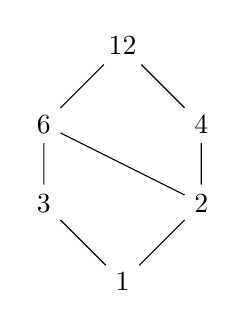
\begin{tikzpicture}
			\node (x12) at (0,3) {$12$};
			\node (x6) at (-1,2) {$6$};
			\node (x4) at (1,2) {$4$};
			\node (x3) at (-1,1) {$3$};
			\node (x2) at (1,1) {$2$};
			\node (x1) at (0,0) {$1$};
			\draw (x12) -- (x4) -- (x2) -- (x1) -- (x3) -- (x6) -- (x12);
			\draw (x2) -- (x6);
			\end{tikzpicture}
			\caption{12}
		\end{minipage}
		\begin{minipage}[b]{0.3\textwidth}
			\centering 
			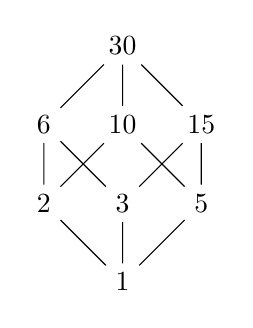
\begin{tikzpicture}
			\node (x30) at (0,3) {$30$};
			\node (x6) 	at (-1,2) {$6$};
			\node (x10) at (0,2) {$10$};
			\node (x15) at (1,2) {$15$};
			\node (x2)  at (-1,1) {$2$};
			\node (x3)  at (0,1) {$3$};
			\node (x5)  at (1,1) {$5$};
			\node (x1)  at (0,0) {$1$};
			\draw (x30) -- (x6) -- (x2) -- (x1) -- (x5) -- (x15) -- (x30);
			\draw (x30) -- (x10) -- (x2);
			\draw (x6) -- (x3) -- (x1);
			\draw (x10) -- (x5);
			\draw (x15) -- (x3);
			\end{tikzpicture}
			\caption{30}
		\end{minipage}
	\end{figure}
\end{sol}

\begin{hw}
Determine the number of non-isomorphic partial orders on $[1]$, $[2]$, $[3]$, $[4]$, (and extra, $[5]$,) respectively.
\end{hw}

\begin{sol}
	Let $f([n])$ be the answer for $[n]$. Then
	$$
	f([1]) = 1, f([2]) = 2, f([3]) = 5, f([4]) = 15
	$$
\end{sol}

\begin{hw}
In class we proved both Dilworth theorem and a dual theorem: In a poset the maximum size of an anti-chain equals the minimum
number of chains that can cover the set; the size of the longest chain equals the minimum number of anti-chains that can cover the set.

Deduce the following Erd\H{o}s-Szekeres theorem from each of the theorems above:

In a sequence of $mn+1$ distinct real numbers, we can always find a subsequence of length $m+1$ that is increasing, or
 a subsequence of length $n+1$ that is decreasing.
\end{hw}

\begin{sol}
	
\end{sol}

\begin{hw} 101 distinct (closed) segments on a line, prove that either there are 11 pairwise disjoint segments, or one can find a point that lies in at least 11 segments. How can you deduce this from Dilworth's theorem?
\end{hw}

\begin{hw}
Let $G=(V, E)$ be a graph whose chromatic number is $k$,
and let $\phi: V \to [k]$ be a proper vertex colouring with exactly
$k$ colours. Prove that we can always find in $G$ a path
$(p_1, p_2, \dots, p_k)$ so that $\phi(p_i) = i$ for all $1 \leq i \leq k$.
\end{hw}

\section{Still haunting}

\begin{hw}
Consider all the permutations on $[100]$ and their cycle
representations.
Let $N$ be the number of those permutations with
exactly 50 cycles. What is $N \mod 3$? Prove your answer.
\end{hw}

\begin{hw}
Prove that, for any positive integer $k$, there exists
a graph whose chromatic number is $k$, yet it does not
contain a triangle.
\end{hw}

\section{Still open}

This is the correct version of the problem I mentioned in class:

\begin{hw} (Open) Given two bipartite graphs $G_1 = (A, B)$ and $G_2 = (A, B)$ such that
  \[ \forall X \subseteq A, |N_{G_1}(X)| \geq |N_{G_2}(X)|.\]
Prove or disprove that the number of $A$-perfect matchings in $G_1$ is no less than that in $G_2$.
\end{hw}

\end{document}
